\documentclass{queriessql}
\titulo{Respondendo 5 perguntas de negócio com SQL}
\autor{Vinicius Olivedo}
\linkedin{vinicius-olivedo}
\urllinkedin{www.linkedin.com}

%\usepackage{lipsum}
% vai gerar um texto aleatório

\begin{document}

\printtitle

%\lipsum[1-2]%chamando o texto aleatório paragrafo 1-2

\begin{comment}
AULA Floats
\lipsum[1]

\begin{table}[!ht]
    \centering
    \caption{Legenda da tabela}
    \begin{tabular}{c|c}
        A & a \\
        B & b
    \end{tabular}
    \label{tab:my_label}
\end{table}

\lipsum[2] 
\end{comment}


\section{Contexto}

    Ao longo dos últimos meses, tenho prestado serviços como \textit{freelancer} no regime de \textbf{home-office}. Ao longo da jornada, foram completos centenas de projetos para clientes ao redor do mundo. No entanto, para aumentar as receitas e entender melhor o negócio, os dados de cada projeto passaram a ser devidamente registrados. Isso permitiu aplicar análise de dados voltada à tomada de decisões, bem como para a obtenção de insights.
    
    Neste documento, mostro um pouco destas análises realizadas na nuvem da \textit{Amazon Web Service} (AWS) e por meio de consultas SQL. O dataset compreendeu 144 projetos registrados. %{\color{BlueViolet}\faBook}


\section{Definições}
\begin{caixa}
    \textbf{Descrição do problema:} busca-se saber a resposta para \destacar{5 perguntas} acerca dos negócios \destacar{freelancer} ao longo de 2020-2022 (atual):
    \begin{enumerate}
            \item Qual foi a receita líquida por ano?
            \item Qual foi o número de projetos completos em cada ano?
            \item Qual é a base de clientes por país?
            \item Qual é a média de valor-hora (em U\$D) por fonte?
            \item Qual é a fonte com mais projetos em cada ano?
    \end{enumerate}
\end{caixa}

\section{Pipeline}
\begin{center}
    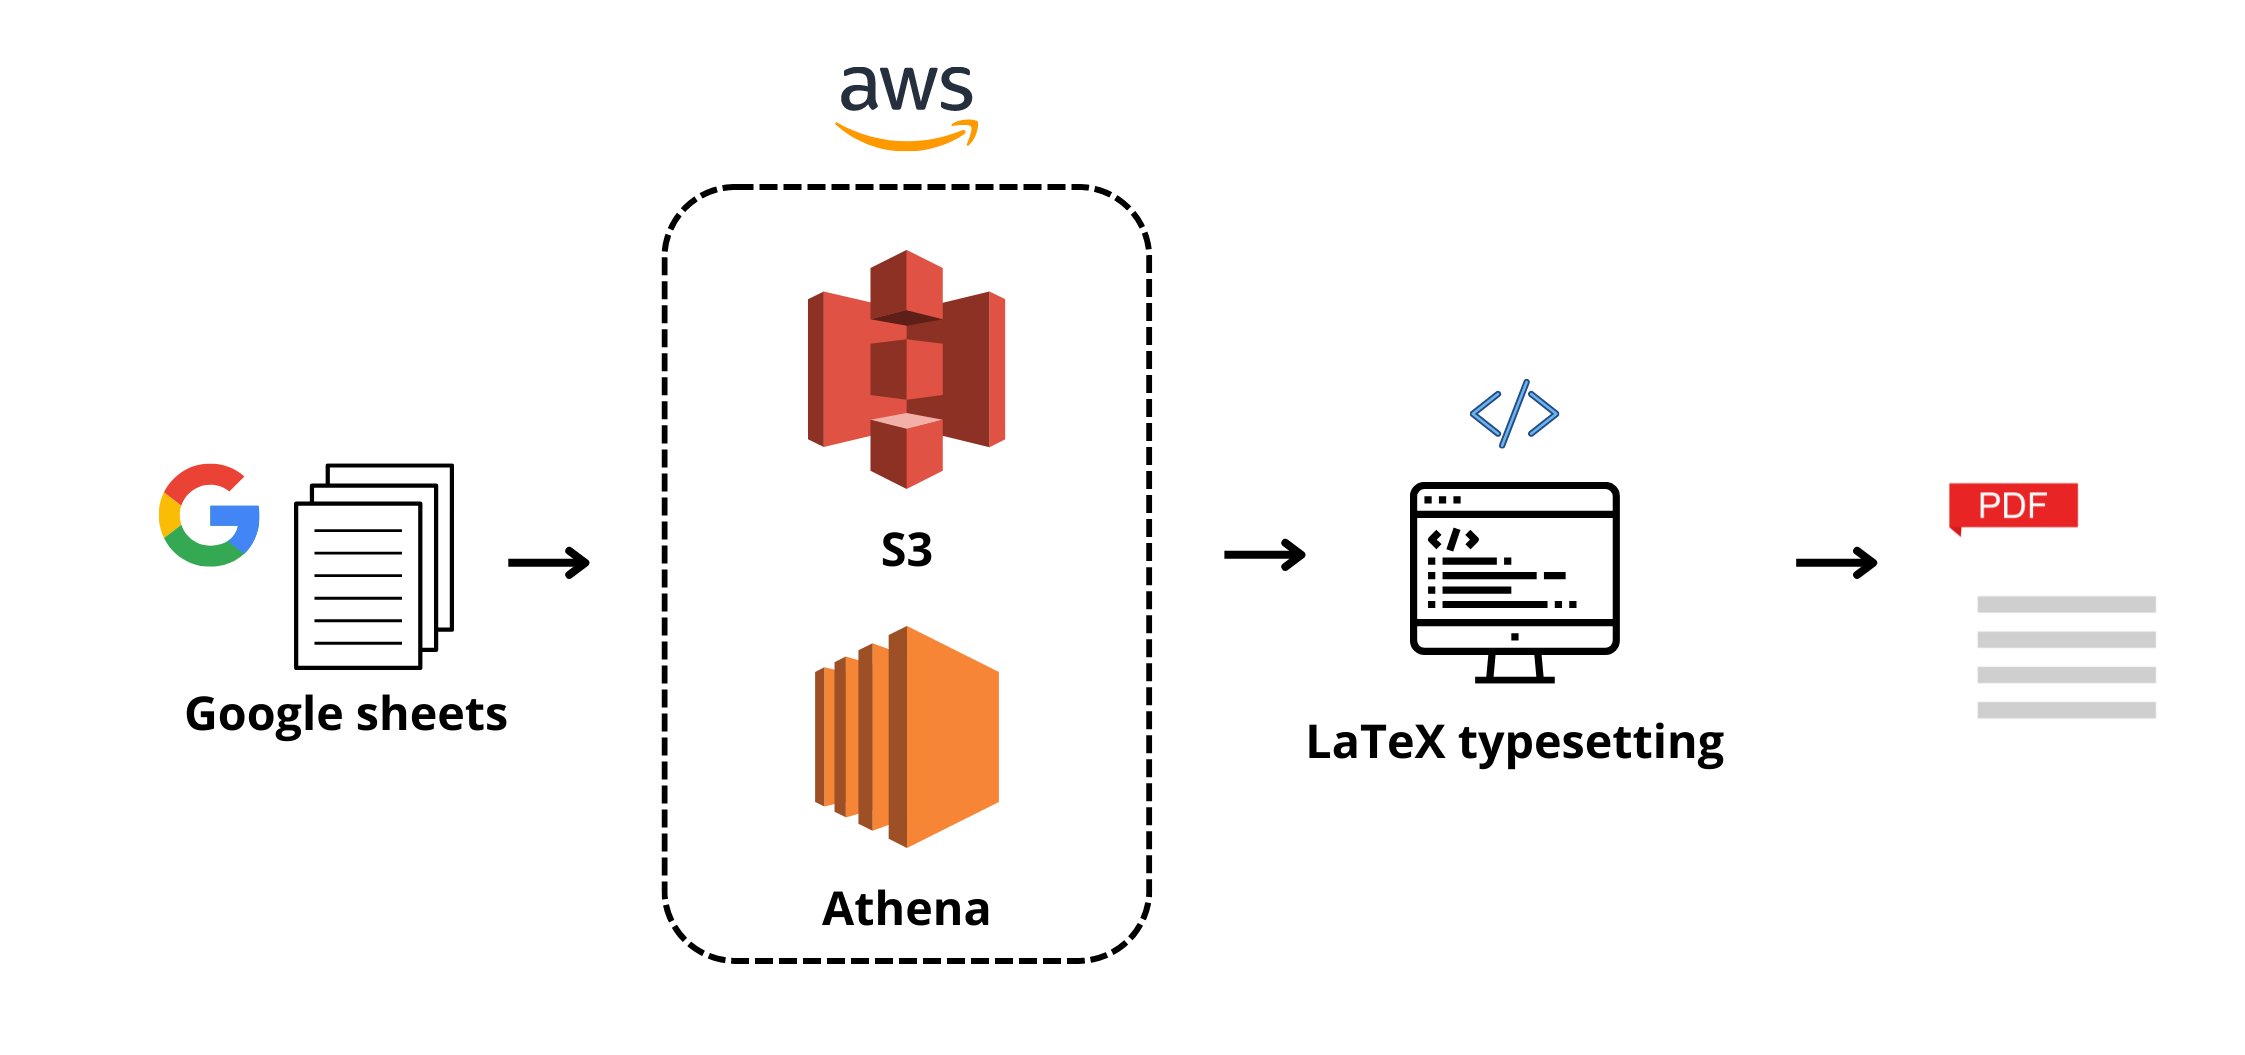
\includegraphics[width=0.9\linewidth]{Figuras/Pipeline-descricao.png}
\end{center}

\clearpage %faz começar na próxima página

\section{Queries}

\subsection{Receita líquida por ano}

\begin{lstlisting}[language=SQL]
SELECT 
    year,
    SUM(amount_earned) as total_earned
FROM 
    projects
GROUP BY 
    year;
\end{lstlisting}


\begin{tabular}{llc}
   \# & \textbf{year} & \textbf{total\_earned} 
      \\ \hline
    1 & 2021 & 5262.530
      \\
    2 & 2022 & 6320.900
      \\
    3 & 2020 & 2686.790
\end{tabular}

\subsection{Projetos completos por ano}

\begin{lstlisting}[language=SQL]
SELECT
    year,
    COUNT(project_id) as projects_completed
FROM    
    projects
GROUP BY year;
\end{lstlisting}


\begin{tabular}{llc}
\# & \textbf{year} & \textbf{projects\_completed} \\ \hline
1 & 2020 & 26 \\
2 & 2021 & 71 \\
3 & 2022 & 47
\end{tabular}


\subsection{Clientes por país:}
\begin{lstlisting}
SELECT 
    country,
    COUNT(country) as customers
FROM projects
GROUP BY country
ORDER by customers DESC;
\end{lstlisting}

\begin{tabular}{llc}
    \# & \textbf{country} & \textbf{customers} \\ \hline
    1 & USA& 60 \\
    2 & Brazil & 20 \\
    3 & UK & 16 \\
    4 & Netherlands & 12 \\
    5 & Germany & 8 \\
    6 & Saudi Arabia & 6 \\
    7 & India & 3 \\
    8 & Spain & 3 \\
    9 & Denmark & 2 \\
    10 & Greece & 2 \\
    11 & Canada & 2 \\
    12 & Finland & 1 \\
    13 & Philippines & 1 \\
    14 & Colombia & 1 \\
    15 & Ireland & 1 \\
    16 & France & 1 \\
    17 & Egypt & 1 \\
    18 & Korea & 1 \\
    19 & Thailand& 1 \\
    20 & Italy & 1 \\
    21 & Belgium & 1
\end{tabular}

\subsection{Valor-hora médio por fonte:}
\begin{lstlisting}
SELECT 
    source,
    AVG(hourly_rate) AS mean_hr
FROM projects
GROUP BY source, year
HAVING year = '2022';
\end{lstlisting}

\begin{tabular}{llc}
    \# & \textbf{source} & \textbf{mean\_hr} \\ \hline
    1 & Direct & 40.29 \\
    2 & Workan & 34.27 \\
    3 & Fiverr & 23.98 \\
    4 & Upwork & 16.88
\end{tabular}

\clearpage %pula pag

\subsection{Fonte com mais projetos completos em cada ano:}
\begin{lstlisting}
SELECT
    year,
    COUNT(project_id) AS projects,
    source
FROM 
    projects
GROUP BY 
    source, year
ORDER BY
    1, 3 DESC;
\end{lstlisting}

\begin{tabular}{llcl}
    \# & \textbf{year} & \textbf{projects} & \textbf{source} \\ \hline
    1 & 2020 & 6 & Study.com \\
    2 & 2020 & 17 & Fiverr \\
    3 & 2020 & 3 & Direct \\
    4 & 2021 & 17 & Study.com \\
    5 & 2021 & 48 & Fiverr \\
    6 & 2021 & 6 & Direct \\
    7 & 2022 & 1 & Workana \\
    8 & 2022 & 1 & Upwork \\
    9 & 2022 & 33 & Fiverr \\
    10 & 2022 & 12 & Direct
\end{tabular}











\end{document}
%%%%%%%%%%%%%%%%%%%%%%%%%%%
\begin{comment}
    \subsection{Subsection}
\lipsum[3]

\subsubsection{Sub-sub}
\end{comment}

\begin{comment} 
    \begin{lstlisting}[language=SQL]%forma 1 de fazer um code listing
  
SELECT 
    id, 
    client_name
FROM clients;

\end{lstlisting}

\lstinputlisting[language=SQL]{query.txt} %forma 2 de fazer code listing (com código em arquivo separado)
\end{comment}
%%%%%%%%%%%%%%%%%%%%%%%%%%